\documentclass[11pt]{article}
\usepackage[left=20mm, right=20mm, top=20mm, bottom=20mm]{geometry} %this sets the page margins 
\usepackage{amsmath}
\usepackage{amsfonts}
\usepackage{amssymb}
\usepackage{graphicx}
\usepackage{wrapfig}
\usepackage{subcaption}
\usepackage[justification=centering]{caption}
\usepackage{setspace}
\doublespacing
\setlength{\parindent}{1cm}
\usepackage{color}
\usepackage{framed}
\usepackage{comment}
\usepackage{pdfpages}
\usepackage{courier}
\usepackage{float}
\usepackage{helvet}
\renewcommand{\familydefault}{\sfdefault}
\usepackage[hyphens]{url}
\usepackage{listings,xcolor}
\usepackage[numbered,framed]{matlab-prettifier}
\renewcommand{\lstlistingname}{Codebox}% Listing -> Algorithm

\newcommand\undermat[2]{%
  \makebox[0pt][l]{$\smash{\underbrace{\phantom{%
    \begin{matrix}#2\end{matrix}}}_{\text{$#1$}}}$}#2}

\numberwithin{equation}{subsection}
\usepackage{titlesec}
\newcommand{\sectionbreak}{\clearpage}

%% THIS BIT MAKES CLICKABLE PDF LINKS
\usepackage{hyperref}
\hypersetup{
    colorlinks,
    citecolor=black,
    filecolor=black,
    linkcolor=black,
    urlcolor=black
}
%%


\author{Henry Fletcher}

\title{Making Flash Memory Work}

%%%%%%%%%%%%%%%%%%%%%%%%%%%%%%%%%%%%%%%%%%%%%%%%%%%%%%%%%%%%%%%%%%%%%%%%%%%%
\begin{document}

\section{Executive Summary}

Modern flash memory is reliant on error-correcting code to ensure error-free operation. Current flash memory architectures often use linear block codes for this purpose (e.g. Reed-Solomon, Hamming or BCH codes). However, the recent rediscovery of LDPC (Low Density Parity Check) codes, which can achieve superior performance close to the Shannon Limit, has generated much interest in the NAND memory industry. These codes could be used to further improve error correction capability in flash memory, thus allowing for more densely packed memory cells and thus larger capacity drives.

The general aim of this project is to produce a MATLAB simulation of how an error correction system using LDPC codes would work for flash memory.  By combining both an error generation and an error correction model, it will be possible to benchmark these rediscovered codes, and subsequently compare them to current generation technologies.

\tableofcontents

\section{Introduction}

\section{Overview of Linear Block Codes}

Linear block codes are one of the two main classes of forward error correction (FEC), with the other main type being convolutional coding. A linear block code essentially takes a block of binary data, and adds additional redundant data onto it. This block can then be transmitted over a noisy channel, and subsequently decoded at the receiver. The redundant bits in the block are used as parity check equations, which allows a linear block code to both detect and correct errors. 

\subsection{Definitions for Linear Block Codes} \label{3.1:definitions}
All linear block codes can be described using a set of standard terms and symbols. For this project, all codes use a binary alphabet of $\{0,1\}$ and hence all operations are over this binary field. $n$ is the block length, the total size of the output codeword. $k$ is the message length, the size of the information vector prior to encoding. An $(n,k)$ error correcting \textit{code} $\mathcal{C}$, will produce a set of $2^k$ output \textit{codewords} $\mathbf{c}$. Hence, $\mathbf{c} \in \mathcal{C}$. 

The rate of any linear block code, $R$, is defined as: 
\begin{equation}
R = \dfrac{k}{n}
\end{equation}
The rate is a measure of the number of information bits compared to the total number of transmitted codeword bits. A high rate code will be more efficient in terms of useful information transmitted, but will have a poorer error correction capability. In Flash Memory, very high rate ($R > 0.9$) codes are used in order to maximise the amount of usable storage space. Conversely, an example use of low rate codes would be in deep-space probe transmissions, where receiving error-free data is more important than rate of transmission.

A linear block code can be represented in two ways: through the $k \times n$ generator matrix $\mathbf{G}$, or the $(n - k) \times n$ parity check matrix $\mathbf{H}$. Each is the null-space of the other, such that:
\begin{equation}
\mathbf{G H}^\top = 0
\end{equation}
Unsurprisingly, the generator matrix $\mathbf{G}$ is used in the transmission side when encoding data, and the parity check matrix $\mathbf{H}$ is used at the receiver to detect and correct any errors.

At the transmitter, if we take a $1 \times k$ input vector of binary data $\mathbf{x}$, the method of encoding this data into a codeword $\mathbf{c}$, is simply a multiplication operation:
\begin{equation}
\mathbf{c = xG}
\end{equation}
At the receiver, a similar operation is performed:
%%%% CHECK THAT THIS IS CORRECT !!! %%%%%
\begin{equation}
\mathbf{s = c H}^\top
\end{equation}
where $\mathbf{s}$ is known as the \textit{syndrome}. If the syndrome is the all zero vector, then error free transmission has occurred. Conversely, if any bit of the syndrome is 1, then this represents a particular error pattern. For small block lengths, these error pattern's can be pre-calculated and saved as a table, allowing for syndrome lookup decoding. The table identifies the exact location of a bit error in the codeword, which can then be `flipped' in order to perform error correction.

An example of a \textit{systematic} generator matrix, in this case a matrix known as the \textit{Hamming(7,4) code}, takes the form:
\begin{equation}
\mathbf{G} = 
\left(
\begin{array}{ccc|cccc}
  1 & 1 & 0 & 1 & 0 & 0 & 0 \\
  0 & 1 & 1 & 0 & 1 & 0 & 0 \\
  1 & 1 & 1 & 0 & 0 & 1 & 0 \\
  %1 & 0 & 1 & 0 & 0 & 0 & 1 \\
  \undermat{n-k}{1 & 0 & 1} & \undermat{k}{0 & 0 & 0 & 1} \\
  \end{array}
\right)
\end{equation}
\\
In this code, 4 information bits are encoded into 7 output bits.
Notice the identity matrix in the right portion of the generator matrix. This means that the 4 message ($k$) bits are always encoded at the end of the codeword, with the parity check ($n-k$) bits at the start of the codeword. This is why it is \textit{systematic}. At the decoder, it is then easy to extract the (uncorrected) message bits from the codeword, simply by looking at the last 4 bits.

\subsection{Hamming weight, distance, and error correction capability}

An important metric when discussing error correcting codes is the concept of the Hamming weight. 
For any codeword, the Hamming weight is defined as the total number of non-zero elements in a given codeword. 
Another metric, the minimum weight ($w_{min}$), is simply the minimum value from the set of all Hamming weight's for a given code, excluding the all-zero case.

\textbf{Example:}
A fictional example (6,2) code could have the following codewords:

\begin{center}
\begin{tabular}{ c | c | c }
Message (2 bits) & Codeword (6 bits) & Hamming weight \\
\hline
0 0 & 0 0 0 0 0 0 & 0 \\
0 1 & 1 0 1 0 1 0 & 3 \\
1 0 & 0 0 1 1 0 0 & 2 \\
1 1 & 1 0 0 1 1 0 & 3 \\
\end{tabular}
\end{center}
For this code, the minimum weight ($w_{min}$) is 2, since that is the smallest value of the Hamming weight's excluding the all-zero case.

Another metric used is the Hamming distance. The Hamming distance defines how `close' any two codewords are to each other. Codewords that are `far away' from each other are less likely to be decoded in error, and hence the Hamming distance determines how `good' a code is at error detection and correction. Formally, the Hamming distance is defined as the number of (binary) places that any 2 codewords differ. Analogous to the minimum weight, there is also a minimum distance ($d_{min}$), which is the minimum value from the set of all Hamming distances for a given code, excluding the trivial case of comparing a codeword to itself.

An important result arises because of the use of binary arithmetic, in that the minimum Hamming weight is in fact equal to the minimum Hamming distance:
\begin{equation}
d_{min} = w_{min}
\end{equation}

It is now possible to present the results that describe, for linear block codes, their error correction and detection performance:

\medskip
\noindent
\textbf{Error Detection Theorem:}
\textit{A linear block code with minimum weight $w_{min}$ is able to detect up to $e$ errors:}
\begin{equation}
e_{detectable} = w_{min} - 1
\end{equation}

\noindent
\textbf{Error Correction Theorem:}
\textit{A linear block code with minimum weight $w_{min}$ is able to correct up to $e$ errors:}
\begin{equation}
e_{correctable} = \dfrac{w_{min} - 1}{2}
\end{equation}

\subsection{Low Density Parity Check codes}
A particular class of codes, known as ``Low Density Parity Check" (LDPC) codes, are of particular interest and relevance to this project. LDPC codes are generally considered to be some of the best performing linear block codes available, in terms of error performance, with some codes getting within a fraction of the Shannon Limit. Additionally, LDPC codes have no patent and hence no licensing costs, making them attractive for real world use.(??!).

LDPC codes were originally discovered by R.G. Gallager in 1962. Then known as ``Gallager codes", they were defined by a sparse parity check matrix with low column weights. Gallager also worked on a probabilty based decoding method for these codes, which proved to have promising performance. However for various reasons, these codes were essentially lost in favour of other more practical codes. It is possible that the decoding complexity for LDPC was, at the time, too great for the computational power then available.\footnote{Personal opinion. Even today, decoding LDPC using near-optimum belief propagation on a PC is computationally expensive, whilst on dedicated ASIC hardware consumes large amounts of power.}

Modern LDPC codes were re-discovered by J.C. MacKay in 1996. MacKay demonstrated that LDPC codes could be decoded using probabilistic methods, even beyond the bound set by their minimum distance. Today, LDPC codes are seeing a resurgence in various applications. Most notably in the DVB-S2 standards for digital HD satellite broadcast, 10GBase-T Ethernet and as optional `add-ons' to the 802.11n/ac wi-fi standards.

Disadvantages of LDPC include the fact that there still exists a small (often in the region of $10^{-6}$ to $10^{-9}$) probability of error after decoding, known as the `error-floor'. This can be avoided by using a second high rate, `inner' Error Correcting Code such as BCH or Reed-Solomon to remove the last few bit errors. Other issues include decoding complexity. Whilst decoding time is linear with block length, decoding using the belief propagation algorithm is still problematic, especially for low power mobile devices. Most applications of LDPC so far have been on mains-powered equipment.


\textbf{Example:}
A specific DVB-S2 code, with $n = 64800$ and $r = 0.9$, has a total of $194,399$ non-zero elements in it's parity check matrix $\mathbf{H}$. However, the non-zero elements account for just 0.04\% of the total matrix: The vast majority of $\mathbf{H}$ is empty. It is therefore easy to see why they are called ``Low Density". In this project, this specific high-rate code is used extensively, especially when modelling the memory-specific case in section ?????????.

\section{Overview of Flash Memory Technology} 

\section{Decoding of LDPC Codes}
Using syndrome lookup decoding as described in section \ref{3.1:definitions} would be nearly impossible for longer block lengths. There is a much better, iterative decoding method that can be used for any linear block code, and which is linear in block length. It is called the belief propagation algorithm (also known as the sum-product algorithm or the message passing algorithm). 

There are two distinct methods of belief propagation: Hard decision decoding and soft decision decoding. In hard decision decoding, the error correction algorithm only receives binary data (i.e. \{1,0\}). In soft decision decoding, the error correction algorithm receives a numerical likelihood of the data being either a 0 or 1. Soft decision decoding will therefore result in superior performance, since it is able to make use of the additional 'soft' information that is otherwise discarded.

\begin{figure}[h]
\centering
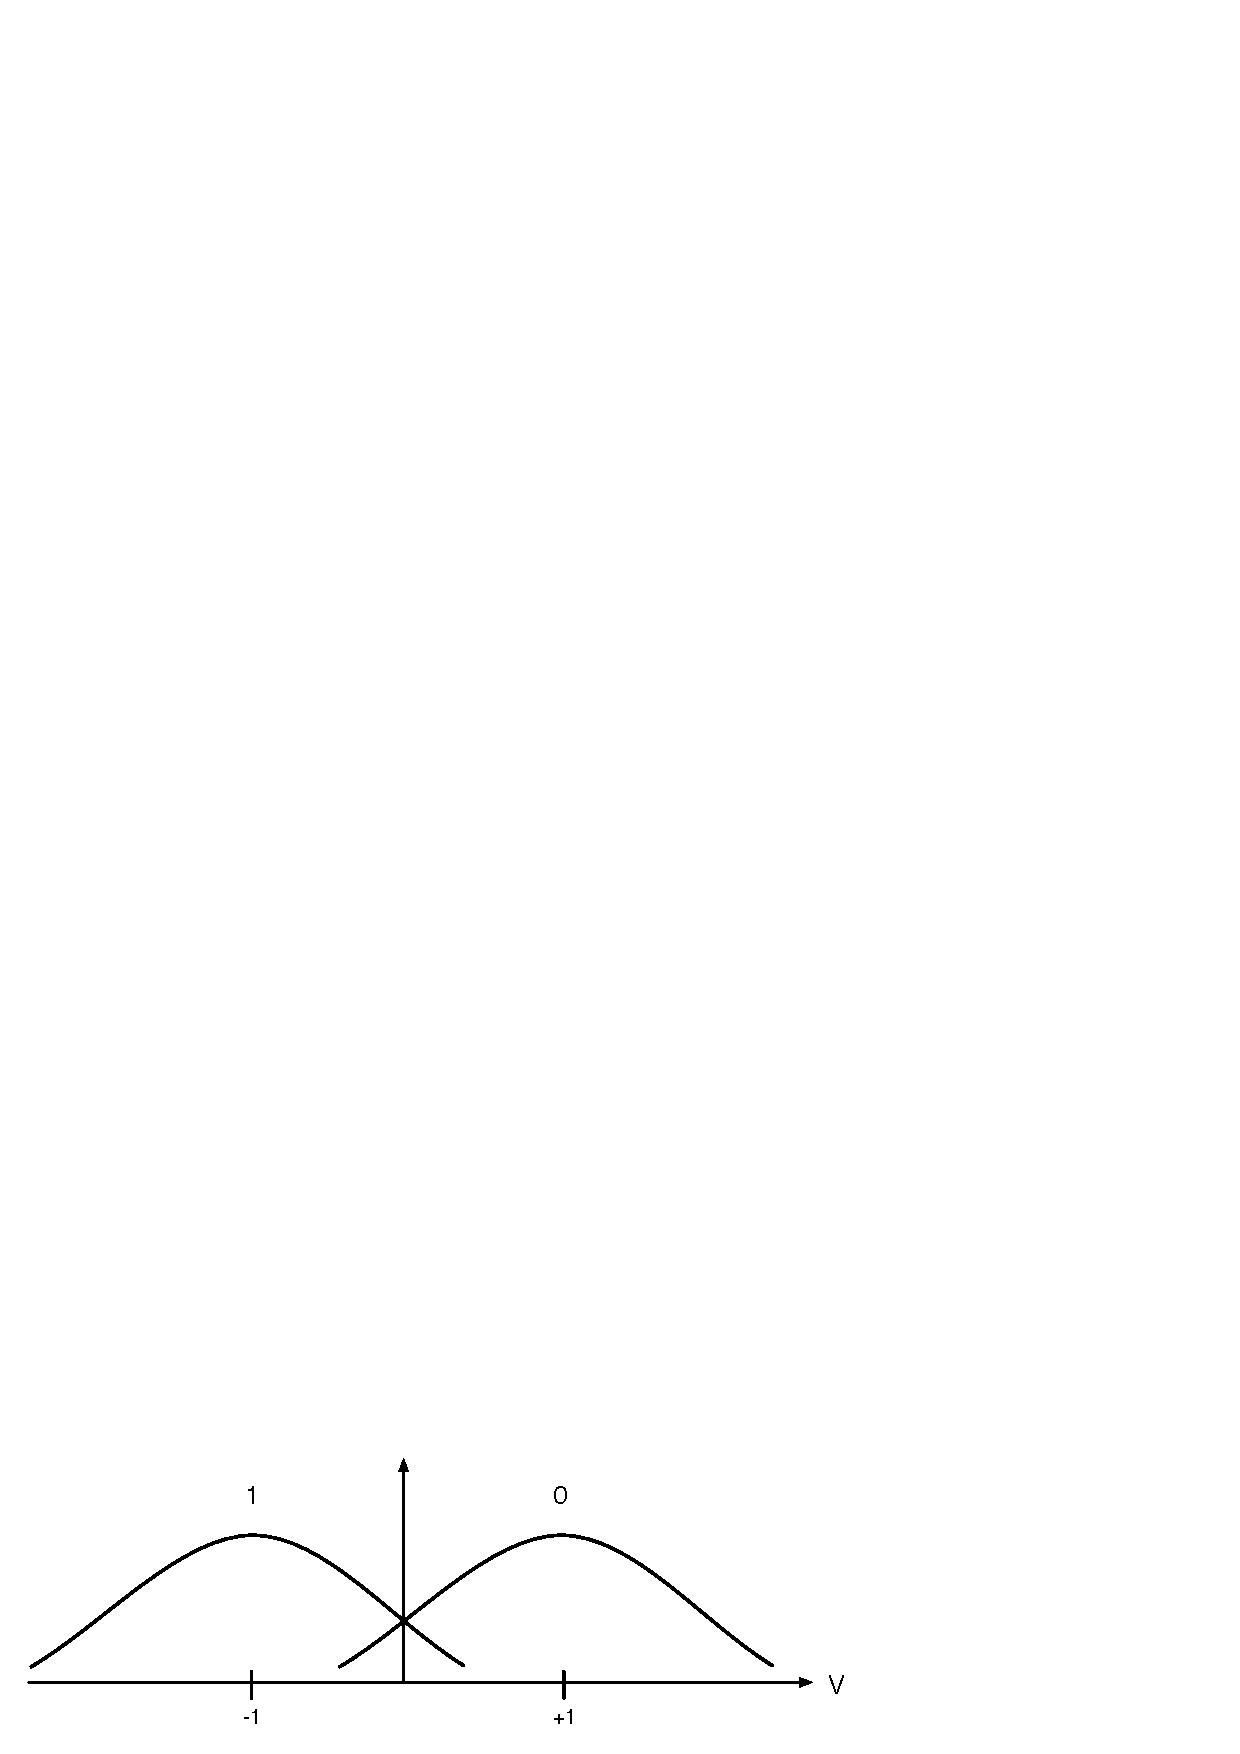
\includegraphics{BPSK_channel_graph}
\caption{Received voltage probability distribution for AWGN channel}
\label{figure:awgn probability graph}
\end{figure}

Figure \ref{figure:awgn probability graph} shows the typical probability distribution of a Binary Phase Shift Keying (BPSK) system with Additive White Gaussian Noise (AWGN). The x-axis is effectively a received voltage value from the demodulator. At transmission, a value of +1 volts corresponds to a binary 0, and a value of -1 volts corresponds to a binary 1. However, the additive noise in the channel results in the received voltage taking a range of values, and hence the received voltage is now defined as a probability distribution.

With hard decision decoding, the obvious boundary would be $x = 0$, half way between the +1 and -1 constellation symbols. Any value to the right side of this boundary would always be classified as binary 0, and anything to the left always binary 1. This means that a voltage value of 0.01 would be output as a binary 0, even though in practice it is almost equiprobable to be a binary 1. The fact that it could equally be a binary 0 or binary 1 is lost when making a hard decision, and the error correction decoder does not get that additional information.

Soft decision decoding seeks to improve on hard decision decoding, by making use of the actual received voltage value, rather than discarding it. The messages are now the conditional \textit{probabilites} of being a 1 or 0, instead of being just binary values. This allows the error correction decoder to know the degree of certainty that the message sent was a 1 or a 0.

\subsection{Hard decision decoding}
The belief propagation algorithm can be best understood with hard decision decoding. As an example, eq \ref{8,4 code} shows the parity check matrix $\mathbf{H}$ of an (8,4) code. This code can also be displayed, as in figure \ref{figure:tanner graph}, as a visual graph representation known as a tanner graph. [Reference: LDPC Leiner tutorial]

\begin{equation} \label{8,4 code} 
\mathbf{H} = 
\left(
\begin{array}{cccccccc}
  0 & 1 & 0 & 1 & 1 & 0 & 0 & 1 \\
  1 & 1 & 1 & 0 & 0 & 1 & 0 & 0 \\
  0 & 0 & 1 & 0 & 0 & 1 & 1 & 1 \\
  1 & 0 & 0 & 1 & 1 & 0 & 1 & 0 \\
\end{array}
\right)
\end{equation}

\begin{figure}[h]
\centering
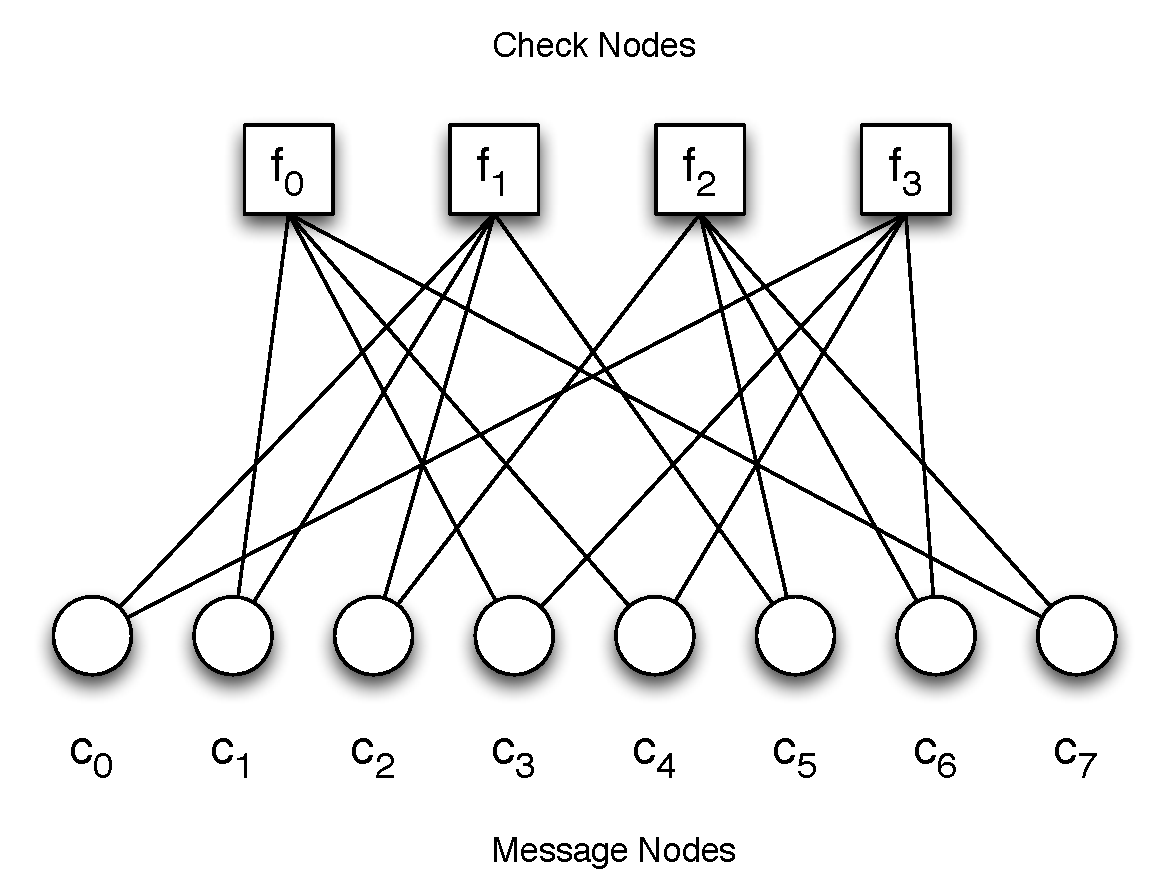
\includegraphics[scale=0.6]{tannergraph}
\caption{Tanner Graph}
\label{figure:tanner graph}
\end{figure}

The tanner graph is a bipartite graph with 2 types of node: Check nodes and Message nodes. The check nodes represent the $(n-k)$ parity check equations, whilst the message nodes represent the $n$ codeword bits. It is directly related to $\mathbf{H}$: Check node $f_i$ connects to message node $c_j$ if element $h_{ij}$ is $1$.

\section{The AWGN channel: Simulation \& Results}
\subsection{Random number generation}
When performing any sort of Monte Carlo simulation, and particularly if running the same program in parallel across multiple computers, it is important to ensure that the random numbers being generated are as random as possible. Even more crucially, there must be no dependence between the parallel task's random numbers if we are to combine result sets.

MATLAB, like many other software packages, cannot generate truly random numbers. Instead, it uses a pseudo-random number generator, such as the Mersenne Twister algorithm. This is just a function that produces numbers which, for most purposes, are considered to be pseudo-random and pseudo-independent. That is, if you generate numbers from this algorithm, they will appear to be random samples from a uniform distribution. 

However, the Mersenne Twister algorithm actually has a finite period. After generating $2^{19937}$ random numbers, the output begins to repeat itself. More importantly, every time MATLAB starts, the random generator is reset to the same position. This means if you try to generate a large set of random numbers in MATLAB, you will always get exactly the same numbers. Effectively, MATLAB uses the same \textit{seed} to the random number generator on every start-up. This is meant to be useful for debugging purposes, however when running simulations in parallel, it causes all the result to no longer be independent. This means you cannot combine results made in parallel, since the output from each parallel stream will actually be identical.

The solution is to ensure that every task executed in parallel has a random seed fed into the random number generator. Effectively, the seed is used as the starting position for the Twister algorithm. If the seed is a truly random number, then each random generator should start in a different position. Any two random generators might start with billions of positions between them, or possibly right next to each other. But the chances of an identical start position are negligible.

\begin{lstlisting}[float=ht,style=Matlab-editor,caption = {Seeding random generator},label=code:rng]
% Ensures truly random numbers for each process
% seed is now a random number that can be used to initialise rand
fid = fopen('/dev/random');
seed = fread(fid, 1, 'uint32');
RandStream.setDefaultStream(RandStream('mt19937ar','seed',seed));
\end{lstlisting}

The commands in codebox \ref{code:rng} were used to seed the random number generator every time a new MATLAB process was created. On UNIX machines, there is a system random number source \mbox{`/dev/random'}, which ``gathers environmental noise from device drivers and other sources into an entropy pool [and] from this entropy pool random numbers are created." The numbers generated by this process originate from physical random processes such as hardware noise, and so it is assumed that when calling the function on a different machine, a different random number will be generated every time. These random numbers are then used to seed the pseudo-random stream in MATLAB. 

\section{Modelling a memory-specific noise channel}

\section{Decoding in the non-Gaussian case}

\section{The memory channel: Simulation \& Results}

\section{Conclusions}

\end{document}